\section{Experimento Bernoulli y distribución binomial}


\subsection{La Distribución Bernoulli y Binomial}


 Si $p$ es la probabilidad de que en un solo ensayo ocurra un evento (llamada la probabilidad de éxito) y $q = 1 - p$ es la
probabilidad de que este evento no ocurra en un solo ensayo (llamada probabilidad de fracaso), entonces la probabilidad de que el evento ocurra exactamente $x$ veces en $N$ ensayos (es decir, que ocurran $x$ éxitos y $N - x$ fracasos) está
dada por
\begin{align}
 \label{eq:2.10.1}
 f(x)=P(X=x)=\comb{N}{x}p^{x}q^{N-x}
\end{align}
donde $x=0,1,...,N.$


 \begin{ejemplo}
  \label{exmp:2.10.1}
  La probabilidad de obtener exactamente dos caras en seis lanzamientos de una moneda es
  \begin{align}
   \comb{6}{2}\left( \dfrac{1}{2} \right)^{2}\left( \dfrac{1}{2} \right)^{6-2}=\dfrac{15}{64}
  \end{align}
empleando \eqref{eq:2.10.1} con $N=6, x=2, p=q=\frac{1}{2}.$
 \end{ejemplo}



\begin{ejemplo}
 \label{exmp:2.10.2}
 Calcule la probabilidad de obtener al menos 4 caras en 6 lanzamientos de una moneda.
\end{ejemplo}

\begin{solucion}
	Usando la distribución binomial con $N=6$, $p=\frac{1}{2}$, $q=\frac{1}{2}$:
	\begin{align}
		P(X \geq 4) &= P(X=4) + P(X=5) + P(X=6) \\
		&= \comb{6}{4}\left(\frac{1}{2}\right)^4\left(\frac{1}{2}\right)^2 + \comb{6}{5}\left(\frac{1}{2}\right)^5\left(\frac{1}{2}\right)^1 + \comb{6}{6}\left(\frac{1}{2}\right)^6 \\
		&= \frac{15}{64} + \frac{6}{64} + \frac{1}{64} = \frac{22}{64} = \frac{11}{32} \approx 0.344
	\end{align}
\end{solucion}



 En lo subsecuente, daremos por hecho que hemos importado los siguientes paquetes:
 \begin{itemize}
  \item \texttt{scipy.stats}
  \item \texttt{numpy} como \texttt{np}
 \end{itemize}


\lstinputlisting[language=Python]{../code/distribuciones-especiales/statsBinom.py}


 \begin{ejemplo}
  \label{exmp:2.10.3}
  Desarrolle $\left( p+q \right)^{4}.$
 \end{ejemplo}


\lstinputlisting[language=Python]{../code/distribuciones-especiales/coefBinom.py}


{Propiedades de la distribución binomial} Supongamos que realizamos $N$ experimentos con probabilidad éxito $p$ y de fracaso $q=1-p.$
\begin{align}
 \label{eq:2.10.2}
 \mu = Np \\
 \label{eq:2.10.3}
 \s^{2}=Npq
\end{align}


\lstinputlisting[language=Python]{../code/distribuciones-especiales/histBinom.py}




 \begin{figure}
 \centering
 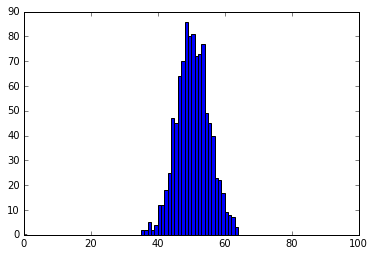
\includegraphics[height=7cm,keepaspectratio=true]{./pe/distBin01.png}
 % distBin01.png: 0x0 pixel, 300dpi, 0.00x0.00 cm, bb=
 \label{fig:2.10.1}
\end{figure}

